% Milling example: part drawing from the part-program (dimensions in mm)
\documentclass[dvisvgm,tikz,border=4pt]{standalone}
% Shared preamble for the TikZ figures in images-1/src (compiled by build.sh)
\usepackage{helvet}
\renewcommand\familydefault{\sfdefault}
\usepackage{amsmath, amssymb}
\usetikzlibrary{arrows.meta, calc, decorations.pathreplacing, patterns, positioning, shapes.geometric, 3d, perspective, fit, backgrounds}
% palette shared with slides.scss and the Graphviz diagrams
\definecolor{dmred}{HTML}{880000}
\definecolor{dmblue}{HTML}{000088}
\definecolor{dmgreen}{HTML}{008800}
\definecolor{dmorange}{HTML}{E08A1E}
\definecolor{ink}{HTML}{333333}
\definecolor{fillblue}{HTML}{E8E8F8}
\definecolor{fillred}{HTML}{F3EAEA}
\definecolor{fillgreen}{HTML}{E8F4E8}
\definecolor{fillorange}{HTML}{FDF0DC}
\definecolor{steel}{HTML}{C9D3DC}
\definecolor{steeldk}{HTML}{8FA3B5}
\definecolor{metal}{HTML}{D9D9D9}
\definecolor{metaldk}{HTML}{A6A6A6}
\tikzset{
  >={Stealth[length=7pt]},
  every picture/.style={line cap=round, line join=round, font=\large},
  proj/.style={gray, dashed, thin},
  dim/.style={<->, >={Stealth[length=5pt]}, thin},
  ext/.style={very thin, gray},
  callout/.style={gray!70!black, thin},
  % datum (origin) symbol
  % pics use absolute sizes so they look the same in mm-scaled drawings
  datum/.pic={
    \fill[white] (0,0) circle (0.22cm);
    \fill[black] (0,0) -- ++(0.22cm,0) arc[start angle=0, end angle=-90, radius=0.22cm] -- cycle;
    \fill[black] (0,0) -- ++(-0.22cm,0) arc[start angle=180, end angle=90, radius=0.22cm] -- cycle;
    \draw[thick] (0,0) circle (0.22cm);
  },
  % reference symbols (absolute sizes): origins have a double circle with a filled quadrant
  wporigin/.pic={
    \draw[thick, fill=white] (0,0) circle (0.3cm);
    \fill[black] (0,0) -- (0.18cm,0) arc[start angle=0, end angle=-90, radius=0.18cm] -- cycle;
    \draw[thick] (0,0) circle (0.18cm);
    \draw (-0.3cm,0) -- (0.3cm,0) (0,-0.3cm) -- (0,0.3cm);
  },
  machorigin/.pic={
    \draw[thick, fill=white] (0,0) circle (0.3cm);
    \fill[black] (0,0) -- (-0.18cm,0) arc[start angle=180, end angle=90, radius=0.18cm] -- cycle;
    \draw[thick] (0,0) circle (0.18cm);
    \draw (-0.3cm,0) -- (0.3cm,0) (0,-0.3cm) -- (0,0.3cm);
  },
  supportpt/.pic={
    \draw[thick, fill=white] (0,0) circle (0.15cm);
    \draw (-0.15cm,0) -- (0.15cm,0) (0,-0.15cm) -- (0,0.15cm);
  },
  regpt/.pic={
    \draw[thick, fill=white] (0,0) circle (0.24cm);
    \draw[thick] (0,0) circle (0.15cm);
    \draw (-0.15cm,0) -- (0.15cm,0) (0,-0.15cm) -- (0,0.15cm);
  },
  % support / registration point (generic)
  target/.pic={
    \draw[thick, fill=white] (0,0) circle (0.12cm);
    \draw (-0.2cm,0) -- (0.2cm,0) (0,-0.2cm) -- (0,0.2cm);
  },
}

\begin{document}
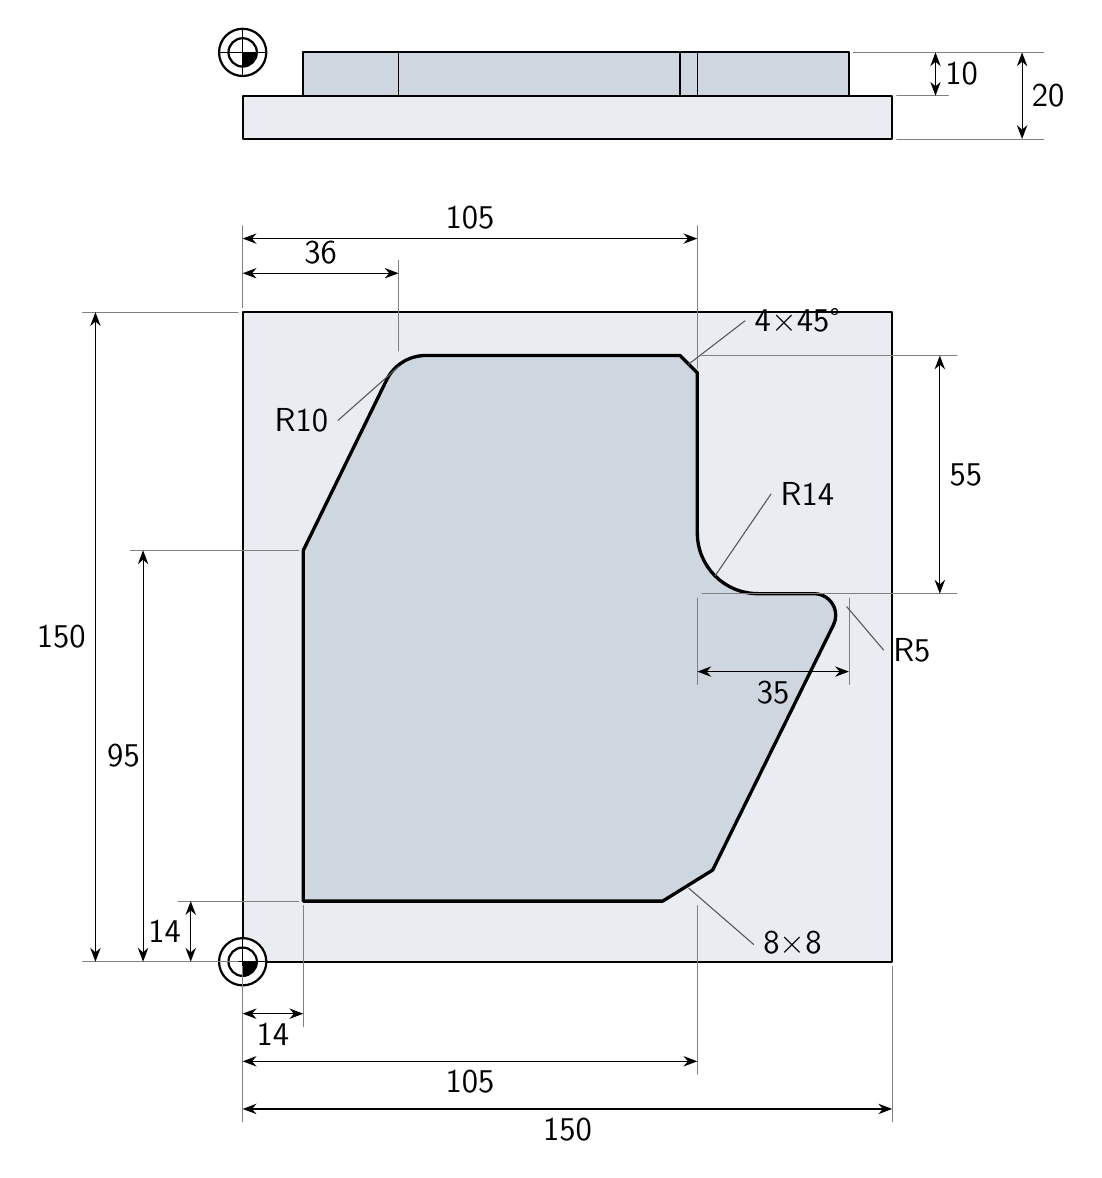
\begin{tikzpicture}[x=0.055cm, y=0.055cm, font=\large]
  % ---------------- top view: stock 150 x 150, island machined 10 mm deep
  \filldraw[thick, fill=steel!40] (0,0) rectangle (150,150);
  \filldraw[very thick, fill=steel!90]
    % rounds: tangent points and arcs computed for R10, R14, R5
    (14,14) -- (14,95)
    -- (33.26,134.39) arc[start angle=153.95, end angle=90, x radius=10, y radius=10]
    -- (101,140) -- (105,136)
    -- (105,99) arc[start angle=180, end angle=270, x radius=14, y radius=14]
    -- (131.96,85) arc[start angle=90, end angle=-26.24, x radius=5, y radius=5]
    -- (108.54,21.17) -- (97,14) -- cycle;
  \pic at (0,0) {wporigin};
  % horizontal dimensions (below and above)
  \draw[ext] (0,-1) -- (0,-37) (14,13) -- (14,-15) (105,13) -- (105,-26) (150,-1) -- (150,-37);
  \draw[dim] (0,-12) -- node[below] {14} (14,-12);
  \draw[dim] (0,-23) -- node[below] {105} (105,-23);
  \draw[dim] (0,-34) -- node[below] {150} (150,-34);
  \draw[ext] (0,151) -- (0,170) (36,141) -- (36,162) (105,137) -- (105,170);
  \draw[dim] (0,159) -- node[above] {36} (36,159);
  \draw[dim] (0,167) -- node[above] {105} (105,167);
  \draw[ext] (106,85) -- (141,85) (140,84) -- (140,64) (105,84) -- (105,64);
  \draw[dim] (105,67) -- node[below] {35} (140,67);
  % vertical dimensions (left and right)
  \draw[ext] (-1,0) -- (-37,0) (13,14) -- (-15,14) (13,95) -- (-26,95) (-1,150) -- (-37,150);
  \draw[dim] (-12,0) -- node[left] {14} (-12,14);
  \draw[dim] (-23,0) -- node[left, fill=white, inner sep=1pt] {95} (-23,95);
  \draw[dim] (-34,0) -- node[left] {150} (-34,150);
  \draw[ext] (106,140) -- (165,140) (141,85) -- (165,85);
  \draw[dim] (161,85) -- node[right] {55} (161,140);
  % rounds and chamfers
  \draw[callout] (36.1,137.5) -- (22,125) node[left, black] {R10};
  \draw[callout] (109.1,89.1) -- (122,108) node[right, black] {R14};
  \draw[callout] (139.5,82) -- (148,72) node[right, black] {R5};
  \draw[callout] (103,138) -- (116,148) node[right, black] {4$\times$45°};
  \draw[callout] (103,17) -- (118,4) node[right, black] {8$\times$8};
  % ---------------- side view
  \begin{scope}[shift={(0,190)}]
    \filldraw[thick, fill=steel!40] (0,0) rectangle (150,10);
    \filldraw[thick, fill=steel!90] (14,10) rectangle (140,20);
    \draw[thin] (36,10) -- (36,20) (101,10) -- (101,20) (105,10) -- (105,20);
    \pic at (0,20) {wporigin};
    \draw[ext] (151,10) -- (163,10) (141,20) -- (185,20) (151,0) -- (185,0);
    \draw[dim] (160,10) -- node[right] {10} (160,20);
    \draw[dim] (180,0) -- node[right] {20} (180,20);
  \end{scope}
\end{tikzpicture}
\end{document}
